\documentclass[11pt]{article}

\usepackage[a4paper,top=30mm,bottom=40mm,left=30mm,right=30mm]{geometry}
\usepackage{pdfpages}
\usepackage[ngerman]{babel}
\usepackage{xcolor}
\usepackage[colorlinks,linkcolor=blue,citecolor=blue]{hyperref}

\author{Raphael Frey, Noah H\"usser}
\title{Briefing Thesis}
\date{\today}

\begin{document}
\maketitle
\section{Aktueller Stand}
\subsection{Evaluation Vorg\"angerprojekt \& Red Pitaya Ecosystem}
\begin{itemize}
    \item Softwareseite  des Red  Pitaya-Projekts ist auf  der Herstellerseite
    stark um  Umbruch (gesamte  Codebasis wird  momentan neu  geschrieben) und
    daher auch ziemlich chaotisch.
    \item  Der alte  Codebranch wird  nicht mehr  maintained und  ist schlecht
    dokumentiert. Er stellt in unserer Ansicht keine zukunftsf\"ahige L\"osung
    dar.
    \item Zitat Entwickler zur neuen Codebase: ``The code is still under heavy
    development and not stable.'' \cite{codebranches}
    \item  Neben der  Codebase selbst  ist auch  die Toolchain  der FPGA-Seite
    nicht gut dokumentiert.
    \item Die  Dokumentation des Linux-Teils des  Pitaya-Projekts scheint aber
    passabel.
    \item Wir  sind uns  nicht sicher, ob  unsere Vorg\"anger  wirklich jemals
    erfolgreicht einen Bitstream auf das FGPA aufgespielt und betrieben haben.
\end{itemize}
\subsection{Entwickeln einer sauberen Toolchain}
\begin{itemize}
    \item Die  Community um den  Red Pitaya  ist ebenfalls nicht  so zufrieden
    mit  der  Dokumentation  des  Projekts. Wir  haben  eine  Person  gefunden
    \cite{pavel}, die  sich daran  gemacht hat, hier  Abhilfe zu  schaffen und
    eine eigene Toolchain am Entwickeln ist.
    \item Diese Toolchain ist ein laufendes Projekt dieser Person, ist modular
    gehalten, einigermassen  gut dokumentiert  (bzw. die  Struktur transparent
    und so aufgebaut, dass sie gr\"osstenteils selbsterkl\"arend ist).
    \item  Daher  sind  wir  nicht   auf  die  (schlechte)  Dokumentation  des
    Pitaya-Projekts angewiesen.
    \item Ebenfalls  sind wir nicht  auf das Fortbestehen  des Pitaya-Projekts
    angewiesen  (es  scheint  etwas   unsicher,  ob  das  Projekt  langfristig
    \"uberlebensf\"ahig).
\end{itemize}

\textbf{Folgerung:} Aufgrund    des    ungeordneten    Zustandes    des
Pitaya-Projekts (insbesondere  der FPGA-Codebase)  scheint uns  eine Grundlage
f\"ur unser Projekt  wichtig, welche nicht mit dem Erfolg  oder Misserfolg des
Pitaya-Projekts selbst steht oder f\"allt.

\begin{itemize}
    \item Wir haben uns daher entschieden, aufbauend auf \cite{pavel} unsere
    eigene Toolchain zu entwickeln. Dies sollte es uns erlauben:
    \begin{itemize}
        \item Nicht  vom Wohlwollen der Pitaya-Entwickler  abh\"angig zu sein.
        \item  Unsere  Toolchain  gr\"undlich  zu  dokumentieren  und  unseren
        Nachfolgern eine saubere  Grundlage sowohl in technischer  wie auch in
        dokumentarischer Hinsicht liefern zu k\"onnen.
    \end{itemize}
    \item Wir haben uns mit der Entwicklungsumgebung f\"ur den Zynq vertraut
    gemacht (Vivado, TCL, ARM Linux).
    \item  Wir  haben TCL-Scripts  von  \cite{pavel}  an unsere  Bed\"urfnisse
    angepasst und ein Blockdesign soweit fertig,  um Daten vom ADC auslesen zu
    k\"onnen.
    \item  Um  dieses  Blockdesign  auf   dem  FPGA  zum  Laufen  zu  bringen,
    m\"ussen wir  ein zugeh\"origes Kernelmodul  auf dem Linux des  Red Pitaya
    installieren. Dies erfordert einen Rebuild  des ARM-Linux des Pitaya. Dies
    ist unser Momentanes Arbeitspaket (``Clean  Linux Build for Pitaya'' unten
    im Zeitplan).
\end{itemize}


\section{Weiteres (geplantes) Vorgehen}

Siehe Zeitplan.

\begin{thebibliography}{1}
    \bibitem{codebranches}
        \href{https://github.com/RedPitaya/RedPitaya/issues/107}        
             {\nolinkurl{https://github.com/RedPitaya/RedPitaya/issues/107}}

    \bibitem{pavel}
        \href{https://pavel-demin.github.io/red-pitaya-notes/}
             {\nolinkurl{https://pavel-demin.github.io/red-pitaya-notes/}}
\end{thebibliography}

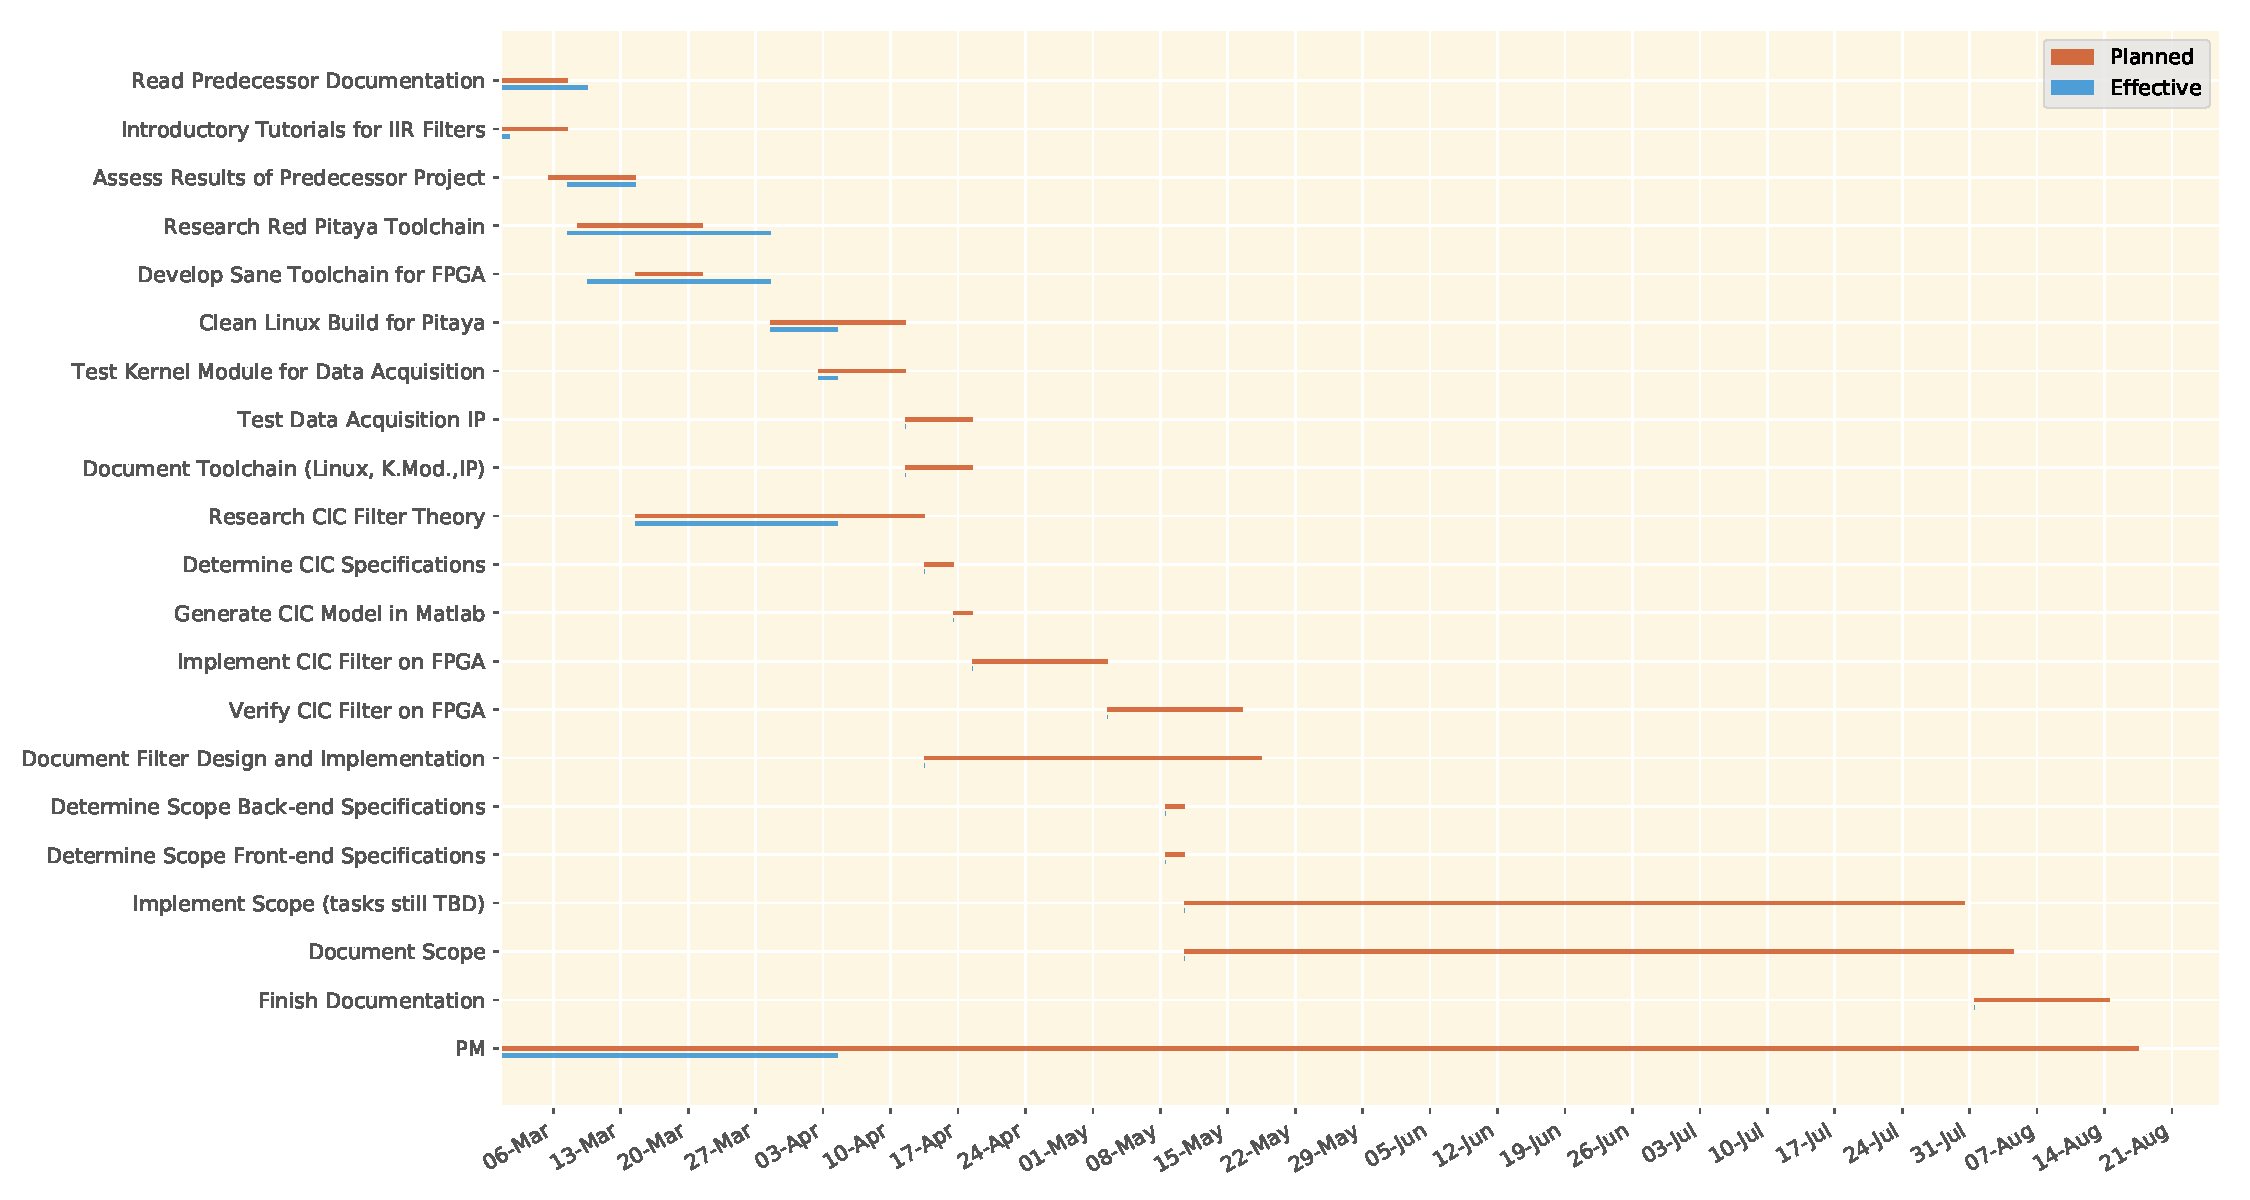
\includepdf[angle=90]{timetable.pdf}
\end{document}
